% Pandoc template for JHEP (jheppub) on the article class. Engine: xelatex (STIX Two).
% Engine: xelatex (STIX Two Text) so the prose Unicode + math render.
\documentclass[11pt,a4paper]{article}
\usepackage{iftex}
\ifPDFTeX
  \usepackage[T1]{fontenc}
  \usepackage[utf8]{inputenc}
\else
  \usepackage{fontspec}
  \setmainfont{STIX Two Text}
\fi

\usepackage{jheppub}   % JHEP: natbib[numbers], amsmath, amssymb, graphicx, hyperref
\usepackage{orcidlink} % ORCID icon next to the author (hyperref already loaded by jcappub)

% --- prose Unicode operators -> math (works under xe/pdf latex) ---
\usepackage{newunicodechar}
\newunicodechar{→}{\ensuremath{\rightarrow}}
\newunicodechar{∂}{\ensuremath{\partial}}
\newunicodechar{∈}{\ensuremath{\in}}
\newunicodechar{∎}{\ensuremath{\blacksquare}}
\newunicodechar{□}{\ensuremath{\Box}}
\newunicodechar{∝}{\ensuremath{\propto}}
\newunicodechar{∞}{\ensuremath{\infty}}
\newunicodechar{∫}{\ensuremath{\int}}
\newunicodechar{≈}{\ensuremath{\approx}}
\newunicodechar{≠}{\ensuremath{\neq}}
\newunicodechar{≡}{\ensuremath{\equiv}}
\newunicodechar{≤}{\ensuremath{\leq}}
\newunicodechar{≥}{\ensuremath{\geq}}
\newunicodechar{≪}{\ensuremath{\ll}}
\newunicodechar{≫}{\ensuremath{\gg}}
\newunicodechar{≲}{\ensuremath{\lesssim}}
\newunicodechar{⊙}{\ensuremath{\odot}}
\newunicodechar{⊗}{\ensuremath{\otimes}}
\newunicodechar{⟹}{\ensuremath{\Longrightarrow}}
\newunicodechar{⟺}{\ensuremath{\Longleftrightarrow}}
\newunicodechar{⇒}{\ensuremath{\Rightarrow}}
\newunicodechar{⇔}{\ensuremath{\Leftrightarrow}}
\newunicodechar{𝓗}{\ensuremath{\mathcal{H}}}
\newunicodechar{√}{\ensuremath{\surd}}
\newunicodechar{∼}{\ensuremath{\sim}}
\newunicodechar{∇}{\ensuremath{\nabla}}
\newunicodechar{↔}{\ensuremath{\leftrightarrow}}
\newunicodechar{⟨}{\ensuremath{\langle}}
\newunicodechar{⟩}{\ensuremath{\rangle}}
\newunicodechar{−}{\ensuremath{-}}
\newunicodechar{ℓ}{\ensuremath{\ell}}
\newunicodechar{ħ}{\ensuremath{\hbar}}
\newunicodechar{′}{\ensuremath{{}^\prime}}
\newunicodechar{Ḣ}{\ensuremath{\dot H}}
\newunicodechar{Ṡ}{\ensuremath{\dot S}}
\newunicodechar{₊}{\ensuremath{{}_{+}}}

% --- pandoc body requirements ---
\usepackage{longtable,booktabs,array}
\usepackage{calc}
\usepackage{float}
\makeatletter
\newsavebox\pandoc@box
\newcommand*\pandocbounded[1]{%
  \sbox\pandoc@box{#1}%
  \Gscale@div\@tempa{\textheight}{\dimexpr\ht\pandoc@box+\dp\pandoc@box\relax}%
  \Gscale@div\@tempb{\linewidth}{\wd\pandoc@box}%
  \ifdim\@tempb\p@<\@tempa\p@\let\@tempa\@tempb\fi%
  \ifdim\@tempa\p@<\p@\scalebox{\@tempa}{\usebox\pandoc@box}%
  \else\usebox{\pandoc@box}%
  \fi%
}
\makeatother
\providecommand{\tightlist}{\setlength{\itemsep}{0pt}\setlength{\parskip}{0pt}}
\graphicspath{{../}{../figures/}}

% --- front matter (jcappub macros) ---
\title{The Scale Sector of a One-Sector Dark Cosmology: μ from
Dimensional Transmutation and Glueball Dark Matter}
\author{Stilian Pandev\,\orcidlink{0009-0005-8153-071X}}
\affiliation{Independent researcher}
\emailAdd{stilianpandev@gmail.com}
\abstract{The SEDE dark-energy law \(\rho_X = \mu^3 H\) requires a mass
scale \(\mu \approx 28.5\) MeV whose origin is the program's
self-declared deepest open problem. We propose that \(\mu\) is the
confinement scale of a hidden \(SU(3)\) sector generated by dimensional
transmutation, and we report the results of a systematic assessment. A
pure hidden Yang--Mills sector confining at \(\mu\) requires
\(\alpha_h(M_{\rm Pl}) = 1/83.2\) --- a log-natural coupling replacing a
\(10^{60}\) tuning, though the exponential map retains sensitivity
\(d\ln\Lambda/d\ln\alpha = 47.5\). A sharper variant, \emph{mirror
unification} (\(\alpha_h(M_{\rm Pl}) = \alpha_s(M_{\rm Pl})\) with
\(N_f = 6\)), introduces \textbf{zero new continuous parameters} and
lands in the right decade: the loop/scheme band is 28--105 MeV at two
loops and 28--133 MeV once three- and four-loop running is included. The
three-loop calculation is deflationary: near the conformal-window edge
the band is irreducibly \(O(1)\)-wide perturbatively, so discriminating
the bare (\(\Lambda_h = \mu\)) from the Urban--Zhitnitsky-corrected
(\(\Lambda_h = 6^{1/3}\mu = 52\) MeV) coefficient is a lattice question.
The dark-energy law itself is inherited via the (contested, unproven)
Urban--Zhitnitsky contact term
\citep{Urban:2009vy, Urban:2009yg, Ohta:2010in}, which remains the
single load-bearing conjecture. The same sector's glueballs supply dark
matter via \(3\to2\) cannibal freeze-out --- a mass miracle, not an
abundance miracle --- with a velocity-independent self-interaction whose
cluster bounds and a conditional Little-Red-Dot seeding bracket
converge, as \emph{constraints}, on \(\Lambda_h \approx 52\) MeV. To
pre-empt an apparent mismatch: the DE-amplitude scale (\(\mu = 28.5\)
MeV) and this DM confinement scale (\(\Lambda_h = 52\) MeV) are the
\emph{same} sector, related by the Urban--Zhitnitsky coefficient
\(\Lambda_h = 6^{1/3}\mu\) --- so \((\Lambda_h/\mu)^3 = 6\) is a
\emph{predicted}, lattice-testable topological factor, not an
independent tuning. We enumerate falsifiers and tag every claim as
derived, matched, or conjectured.}


% absorb small unbreakable-line overruns instead of margin overflow
\setlength{\emergencystretch}{3em}

\begin{document}
\maketitle
\section{Introduction}\label{sec-1}

The parent program of this paper is a one-sector dark cosmology (USC)
joining two constructions through a single horizon-entropy ledger: ECCG,
which generates the matter sector (baryogenesis and, in its original
branch, an asymmetric dark-matter relic at \(m_X = 1.78\) GeV), and
SEDE, which generates dark energy through the law

\begin{equation}\rho_X = \mu^3 H, \qquad \mu \approx 28.5\ \text{MeV}.\end{equation}

Everything in SEDE's phenomenology --- the H-linear equation of state,
the growth gate, the modified-growth signatures --- descends from this
one dimensionful input. The SEDE completion standard (v0.3, item \#5)
names the origin of \(\mu\) as the deepest open problem of the
construction: \(28.5\) MeV corresponds to a vacuum energy density tuned
to one part in \(\sim 10^{60}\) against the Planck scale if put in by
hand.

There is a natural candidate mechanism inside the corpus's own toolkit.
ECCG generates its high scale \(\Lambda_H\) by dimensional transmutation
\citep{Coleman:1973jx} --- the logarithmic running of a dimensionless
gauge coupling from the Planck scale down to a confinement scale.
Transmutation is the only known mechanism that converts an \(O(1)\)
dimensionless input into an exponentially suppressed dimensionful output
without tuning:

\begin{equation}\Lambda = M_{\rm Pl}\, e^{-2\pi / (b_0\, \alpha(M_{\rm Pl}))}.\end{equation}

This paper assesses the proposal that \(\mu\) is the confinement scale
\(\Lambda_h\) of a hidden \(SU(3)\) gauge sector, in two versions of
increasing economy (a postulated coupling; a \emph{mirror-unified}
coupling with no new continuous input), together with the mechanism that
would convert the \emph{scale} into the \emph{law} \(\rho_X = \mu^3 H\)
(the Urban--Zhitnitsky/Ohta topological vacuum energy), and the
observation that the same sector's glueballs are a viable dark-matter
candidate with distinctive, velocity-independent self-interactions.

The law \(\rho_X = \mu^3 H\) is not itself new: it is the
Urban--Zhitnitsky/Ohta QCD-ghost (Veneziano contact-term) dark-energy
law \(\rho_{\rm DE} \propto \Lambda^3 H\)
\citep{Urban:2009vy, Urban:2009yg, Ohta:2010in, Cai:2010uf}, with the
single substitution \(\Lambda_{\rm QCD} \to \Lambda_{\rm hidden}\). Our
contribution is not the law but (i) fixing the scale \(\mu\) by
dimensional transmutation of a hidden \(SU(3)\), and (ii) tying the same
sector to glueball dark matter. Notably the same \(H\)-linear form is
reached from an entirely different route --- a volume-law horizon
entropy gives \(\rho \propto H\) in entropic cosmology
\citep{Komatsu:2015nkb, Komatsu:2012zh}, which is the route the SEDE
cosmology companion takes --- so \(\rho \propto H\) is doubly-motivated
(QCD contact term \emph{and} horizon thermodynamics), a convergence
rather than a coincidence. The parent QCD-topological-sector program
remains active, and is being tested against current cosmological data
\citep{VanWaerbeke:2025shm}.

We are explicit throughout about the provenance of each claim: which
quantities are \emph{derived} (following from stated inputs by a
reproducible calculation), which are \emph{matched} to data (a computed
number compared against an observed or required value), which are
\(O(1)\)-controlled \emph{estimates}, and which are \emph{conjectures}
(a mechanism whose validity is not established). Every numerical claim
below carries its provenance; all are reproducible from the scripts
listed in §\ref{sec-10}.

\begin{center}\rule{0.5\linewidth}{0.5pt}\end{center}

\section{The transmutation mechanism}\label{sec-2}

\subsection{The coupling that does the job}\label{sec-2-1}

For a pure hidden \(SU(3)\) Yang--Mills sector (\(b_0 = 11\)), one-loop
transmutation from the Planck scale gives

\begin{equation}\frac{1}{\alpha_h(M_{\rm Pl})} = \frac{11}{2\pi} \ln\frac{M_{\rm Pl}}{\Lambda_h}.\end{equation}

Setting \(\Lambda_h = \mu = 28.55\) MeV yields

\begin{equation}\frac{1}{\alpha_h(M_{\rm Pl})} = 83.2, \qquad \alpha_h(M_{\rm Pl}) = 0.0120.\end{equation}

This is the same ballpark as the Standard Model couplings at
\(M_{\rm Pl}\) (\(1/\alpha \sim 47\)--\(59\)), though not equal to any
of them. The check verifies exactly
(\texttt{mu\_transmutation\_check.py}). The \(10^{60}\) tuning in
\(\rho\) genuinely becomes a log-natural coupling specification.

We quote here the full Planck mass \(M_{\rm Pl} = 1.22\times10^{19}\)
GeV; the reduced-mass convention gives \(1/\alpha \approx 80\). We
therefore quote \(1/\alpha_h(M_{\rm Pl}) \approx 80\)--\(83\), a
convention band rather than a determination.

\subsection{Sensitivity honesty}\label{sec-2-2}

The transmutation map is exponential, and honesty requires stating its
Jacobian:

\begin{equation}\frac{d\ln\Lambda_h}{d\ln\alpha_h} = \ln\frac{M_{\rm Pl}}{\Lambda_h} = 47.5.\end{equation}

A 1\% specification of \(\alpha_h(M_{\rm Pl})\) fixes \(\mu\) only to
\(\sim 48\%\) (a factor 1.6); pinning \(\mu\) to 1\% would require
\(\alpha_h\) specified to 0.02\%. The correct statement is therefore:
\textbf{transmutation naturalizes the scale; the precise value of
\(\mu\) remains a mild, log-level selection} unless the coupling itself
is fixed by a principle. That principle is the subject of §\ref{sec-3}.

\begin{center}\rule{0.5\linewidth}{0.5pt}\end{center}

\section{Mirror unification: zero new continuous parameters in, an O(1)
band out}\label{sec-3}

\subsection{The construction}\label{sec-3-1}

Rather than postulating \(\alpha_h\), demand that the hidden coupling
\emph{equal the visible QCD coupling at the Planck scale} --- the
coupling-inheritance structure familiar from mirror/twin constructions
\citep{Chacko:2005pe}:

\begin{equation}\alpha_h(M_{\rm Pl}) = \alpha_s(M_{\rm Pl}).\end{equation}

Running the measured \(\alpha_s(M_Z) = 0.1181\) up at two loops (with
the \(N_f\,5\to6\) threshold at \(m_t\)) gives
\(\alpha_s(M_{\rm Pl}) = 0.01886\), i.e.~\(1/\alpha = 53.0\). The hidden
confinement scale is then fixed entirely by the \emph{discrete} flavor
content of the mirror sector. At one loop
(\texttt{mu\_transmutation\_check.py}):

\begin{longtable}[]{@{}
  >{\raggedright\arraybackslash}p{(\linewidth - 2\tabcolsep) * \real{0.5000}}
  >{\raggedright\arraybackslash}p{(\linewidth - 2\tabcolsep) * \real{0.5000}}@{}}
\toprule\noalign{}
\begin{minipage}[b]{\linewidth}\raggedright
hidden \(SU(3)\) content
\end{minipage} & \begin{minipage}[b]{\linewidth}\raggedright
\(\Lambda_h\) (one loop)
\end{minipage} \\
\midrule\noalign{}
\endhead
\bottomrule\noalign{}
\endlastfoot
\(N_f = 0\) & \(1.2\times10^{6}\) MeV \\
\(N_f = 3\) & \(1.6\times10^{3}\) MeV \\
\textbf{\(N_f = 6\)} & \textbf{\(\sim\)30--46 MeV} \\
\(N_f = 7\) & \(0.3\) MeV \\
\end{longtable}

A mirror QCD with six light flavors and a Planck-unified coupling
confines within a factor \(\sim 2\) of \(\mu\), with \textbf{no new
dimensionless inputs}: the coupling is inherited and \(N_f\) is
discrete. This is the strongest form of the proposal, and the ``zero new
continuous parameters'' claim attaches precisely here --- \textbf{to the
input}. It does \emph{not} attach to the output, as the next two
subsections make quantitative.

\subsection{Two-loop refinement: the single number dissolves into a
band}\label{sec-3-2}

The two-loop calculation with thresholds
(\texttt{mu\_transmutation\_steps.py}) supersedes the early one-loop
quote of ``\(\Lambda_h \approx 46\) MeV'':

\begin{longtable}[]{@{}
  >{\raggedright\arraybackslash}p{(\linewidth - 2\tabcolsep) * \real{0.5000}}
  >{\raggedright\arraybackslash}p{(\linewidth - 2\tabcolsep) * \real{0.5000}}@{}}
\toprule\noalign{}
\begin{minipage}[b]{\linewidth}\raggedright
scheme / order
\end{minipage} & \begin{minipage}[b]{\linewidth}\raggedright
\(\Lambda_h\)
\end{minipage} \\
\midrule\noalign{}
\endhead
\bottomrule\noalign{}
\endlastfoot
1-loop pole & \textbf{27.6 MeV} \\
2-loop pole & 105 MeV \\
2-loop \(\overline{\rm MS}\)-form & 88 MeV \\
\emph{(targets)} & bare \(\mu = 28.5\) · UZ-corrected
\(6^{1/3}\mu = 51.9\) \\
\end{longtable}

Two honest conclusions. (i) Mirror unification with \(N_f = 6\)
\textbf{robustly lands in the right decade with zero new continuous
parameters} --- a consistency check that the mirror hypothesis is not
excluded. \(N_f = 6\) is the flavor content selected to land in the
decade (\(N_f = 5, 7\) miss by orders of magnitude); given
\(\alpha_s(M_{\rm Pl}) \sim 1/53\) and
\(d\ln\Lambda/d\ln\alpha \approx 47.5\), hitting the decade was
near-automatic --- a consistency check, not a prediction. (ii) The
loop/scheme spread (\(\times 2\) each way, band \(\approx\) 28--105 MeV)
\textbf{cannot distinguish} the bare coefficient (\(\Lambda_h = \mu\))
from the UZ-corrected one (\(\Lambda_h = 6^{1/3}\mu\), §\ref{sec-4}). An
earlier claim of ``12\% alignment'' with the UZ target was premature and
is retracted: the band brackets \emph{both} targets.

\subsection{The three-loop result: deflationary, and instructively
so}\label{sec-3-3}

The scheme-fixed three-loop (and four-loop) running was computed as
Tier-1 item \#2 (\texttt{mirror\_qcd\_3loop.py}), with the explicit
question of whether it tightens the band. It does not:

\begin{longtable}[]{@{}
  >{\raggedright\arraybackslash}p{(\linewidth - 2\tabcolsep) * \real{0.5000}}
  >{\raggedright\arraybackslash}p{(\linewidth - 2\tabcolsep) * \real{0.5000}}@{}}
\toprule\noalign{}
\begin{minipage}[b]{\linewidth}\raggedright
loop order
\end{minipage} & \begin{minipage}[b]{\linewidth}\raggedright
\(\Lambda_{\rm pole}\)
\end{minipage} \\
\midrule\noalign{}
\endhead
\bottomrule\noalign{}
\endlastfoot
1 & 28 MeV \\
2 & 105 MeV \\
3 & spurious IR fixed point --- \(\beta\) develops a zero at
\(a \approx 0.28\) (\(\alpha \approx 3.5\)), outside perturbative
control \\
4 & 133 MeV \\
\end{longtable}

\textbf{The three-loop does not tighten the band; it reveals why no
perturbative order will.} \(N_f = 6\) \(SU(3)\) sits close enough to the
conformal-window edge (\(N_f^* \sim 8\)--12) that the confinement scale
is loop-order-sensitive: the 1-loop--4-loop span is a factor \(\sim 5\)
(28--133 MeV), and the three-loop \(\beta\)-function's fixed point at
\(\alpha \approx 3.5\) is an artifact appearing where perturbation
theory has already failed. The band is \textbf{irreducibly \(O(1)\)-wide
from perturbation theory} near the conformal edge. This is a negative
refinement of the two-loop result and we present it as such: the
zero-parameter mirror construction brackets \(\mu\) to the right decade
--- a real success --- but perturbation theory \emph{cannot} pin the
value to 28.5 vs 52 MeV.

\begin{figure}
\centering
\pandocbounded{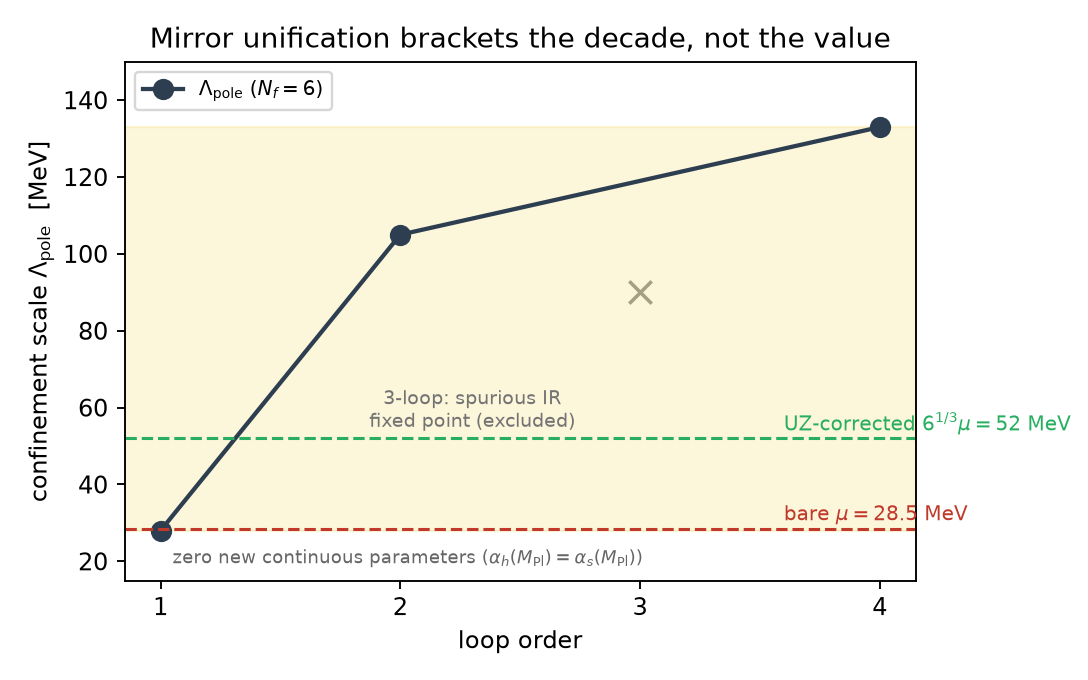
\includegraphics[keepaspectratio]{figures/fig1_mirror_band.png}}
\caption{Mirror unification brackets the decade, not the value. The
confinement scale \(\Lambda_{\rm pole}\) from \(N_f=6\) running, with
zero new continuous parameters
(\(\alpha_h(M_{\rm Pl})=\alpha_s(M_{\rm Pl})\)), spans 28--133 MeV
across loop orders (the three-loop point is a spurious IR fixed point
where perturbation theory has already failed). The band is irreducibly
\(O(1)\)-wide near the conformal-window edge and cannot discriminate the
bare \(\mu=28.5\) MeV from the UZ-corrected \(6^{1/3}\mu=52\) MeV --- a
lattice question (§\ref{sec-3-4}).}\label{fig:1}
\end{figure}

\subsection{\texorpdfstring{The closer: lattice
\(T_c/\Lambda_{\overline{\rm MS}}\) {[}SPECIFIED,
external{]}}{The closer: lattice  {[}SPECIFIED, external{]}}}\label{sec-3-4}

The physical scale requires one nonperturbative \(O(1)\) input: the
ratio \(T_c/\Lambda_{\overline{\rm MS}}\) for \(N_f = 6\) \(SU(3)\). Per
external-calculation spec S-4, this is a pure lattice question with
standard technology (light degenerate quarks, \(T_c\) from the
chiral-susceptibility peak, \(\Lambda_{\overline{\rm MS}}\) via the
gradient-flow coupling); existing near-conformal-window
\(N_f \approx 6\) studies may permit a reanalysis without new runs. The
pre-registered decision rule:
\textbf{\(T_c/\Lambda_{\overline{\rm MS}}\) pins \(\Lambda_h\) within
\(\sim 15\%\), at which point the transmutation \(\mu\) is either 28.5
MeV (bare) or 52 MeV (UZ-corrected)} --- discriminating the two
coefficients that the astrophysical probes of §\ref{sec-7} attack from
opposite sides.

\begin{center}\rule{0.5\linewidth}{0.5pt}\end{center}

\section{From scale to law: the Urban--Zhitnitsky mechanism
(conjectured)}\label{sec-4}

The law \(\rho_X = \mu^3 H\) is not itself new: it is the
Urban--Zhitnitsky/Ohta QCD-ghost (Veneziano contact-term) dark-energy
law \(\rho_{\rm DE} \propto \Lambda^3 H\)
\citep{Urban:2009vy, Urban:2009yg, Ohta:2010in, Cai:2010uf, Cai:2012fq},
with the single substitution
\(\Lambda_{\rm QCD} \to \Lambda_{\rm hidden}\). Our contribution is not
the law but (i) fixing the scale \(\mu\) by dimensional transmutation of
a hidden \(SU(3)\), and (ii) tying the same sector to glueball dark
matter.

\subsection{The mechanism and its contested status}\label{sec-4-1}

Transmutation supplies the \emph{scale}; SEDE needs the \emph{law}
\(\rho_X = \mu^3 H\). The candidate bridge is the Urban--Zhitnitsky/Ohta
proposal \citep{Urban:2009vy, Urban:2009yg, Urban:2009sw, Ohta:2010in}:
in a universe with a finite causal horizon, the topological
(Veneziano-ghost / contact-term) sector of a confining theory shifts the
vacuum energy from its Minkowski value by

\begin{equation}\Delta\rho \sim H \cdot \frac{\chi_{\rm top}}{m_{G}} \sim \frac{H\,\Lambda_h^3}{6},\end{equation}

using the lattice pure-glue relations \(m_G \approx 6\Lambda\) and
\(\chi_{\rm top} \sim \Lambda^4\). The linear-in-\(H\),
boundary-sensitive form is exactly SEDE's law, and it fixes the required
confinement scale not at \(\mu\) but at

\begin{equation}\Lambda_h = 6^{1/3}\mu = 52\ \text{MeV}.\end{equation}

\textbf{Status: conjectural and contested.} The Veneziano ghost is
gauge-variant and non-propagating; whether the linear-in-\(H\) term
survives careful regularization has been debated since \(\sim\)2011 and
is unsettled in the literature
\citep{Garcia-Salcedo:2013htj, Ebrahimi:2011js, Dudal:2015khv}. Within
the transmutation route this is now the single load-bearing assumption,
and we do not soften that: if the UZ term does not survive, the route
delivers a natural scale with no mechanism for the law.

\subsection{The structural argument: UZ as a candidate identity for the
N1 degrees of freedom}\label{sec-4-2}

There is nonetheless a corpus-internal reason to take the mechanism
seriously. The USC gap audit proved a no-go: the volume-law horizon
entropy count \emph{cannot} be the entanglement entropy of local QFT
degrees of freedom (the Casini/Bekenstein bound gives
\(S_{\rm vol}/S_{\rm Bek} = 1/H_0 R\)), forcing \textbf{nonlocal horizon
degrees of freedom} --- node N1, flagged as the program's most important
open structural problem. The Veneziano-ghost/topological sector is
precisely a \textbf{nonlocal, non-propagating, boundary-sensitive
contact term}, not a local propagating QFT mode
\citep{Zhitnitsky:2011tr, Zhitnitsky:2011aa, Thomas:2011ee}. The UZ
mechanism is therefore one candidate in a class of horizon-sensitive
vacuum-energy mechanisms
\citep{Urban:2009vy, Urban:2009yg, Ohta:2010in, Cai:2010uf, Klinkhamer:2009ri, Volovik:2008qub},
all sharing the same regularization controversy; its specific appeal
here is the \(\chi_{\rm top}/m_G\) coefficient, not uniqueness. It
simultaneously (a) produces \(\rho \propto H\Lambda^3\) and (b) has the
nonlocal character N1 demands. It also \emph{evades} (does not violate)
the corpus's Casini-at-all-times theorem, which excludes local processes
producing the horizon count: the contact-term vacuum energy is not local
entanglement by construction. The transmutation proposal is thus not
only a candidate origin for \(\mu\); it is a candidate identity for N1's
mystery degrees of freedom. This is an alignment of structures, not a
derivation, and the mechanism remains a conjecture.

The gate also fits structurally: UZ supplies the \emph{ceiling}
\(\mu^3 H\), and SEDE's activation fraction
\(u = f_{\rm sat} \in [0,1]\) (the foundations paper's ``occupancy''
reading) supplies the timing, driven by the Avrami structure-collapse
coverage. What makes the contact term \emph{gateable} remains the
corpus's open covariant-gate question, unchanged by this proposal.

\subsection{The lattice discharge test {[}SPECIFIED,
external{]}}\label{sec-4-3}

The contested-mechanism question can be converted into a computable
yes/no with no cosmology at all. The UZ claim implies a
finite-volume/boundary dependence of the pure-glue vacuum energy:

\begin{equation}\rho_{\rm vac}(L) - \rho_{\rm vac}(\infty) \propto \frac{\chi_{\rm top}}{m_G\, L},\end{equation}

which is lattice-measurable in principle (pure \(SU(3)\), varying box
size and boundary conditions, target coefficient
\(\chi_{\rm top}/m_G\)). This is the sharpest available discharge path
for the load-bearing conjecture.

\begin{center}\rule{0.5\linewidth}{0.5pt}\end{center}

\section{Glueball dark matter}\label{sec-5}

\subsection{Cannibal freeze-out and the natural coupling}\label{sec-5-1}

The hidden sector confines into glueballs of mass
\(m_G = 6\Lambda_h \approx 180\)--630 MeV across the perturbative band.
Glueballs of a hidden non-Abelian sector are a well-studied dark-matter
candidate
\citep{Boddy:2014yra, Soni:2016gzf, Halverson:2016nfq, Halverson:2018olu},
with the relic abundance and \(\Delta N_{\rm eff}\) set by the confining
sector's cosmology \citep{Forestell:2017wov, Carenza:2023eua}. Pure glue
has no renormalizable portal to the Standard Model, so the operative
relic regime is the \textbf{decoupled cannibal} one
\citep{Carlson:1992fn}: number-changing \(3\to2\) (SIMP-type)
self-annihilations
\citep{Hochberg:2014dra, Hochberg:2014kqa, Hochberg:2015vrg} with
separate hidden-sector entropy, frozen out when \(\Gamma_{3\to2} = H\)
\citep{Pappadopulo:2016pkp, Farina:2016llk, Kuflik:2015isi}. The full
calculation (\texttt{glueball\_simp\_relic.py}: separate-entropy
tracking, Boltzmann-equilibrium cannibalization) confirms the coupling
naturalness: solving for \(\Omega h^2 = 0.12\) requires

\begin{equation}\alpha_{\rm eff} \approx 0.25\text{–}0.6\end{equation}

at the viable points --- exactly what a confining sector at its own
scale supplies. This is a value matched to the required relic abundance,
not an independent prediction.

An earlier exclusion is retracted for this regime: the
``\(\Delta N_{\rm eff} = 0.43 \Rightarrow\) marginally excluded'' result
applied to a hidden sector still \emph{relativistic} at BBN/CMB. Here
confinement at \(T_h \sim \Lambda_h\) converts the gluons to massive
glueballs long before BBN and cannibalization keeps them
non-relativistic: \(\Delta N_{\rm eff} \approx 0\), invisible to CMB-S4.
The dark-radiation channel is therefore \emph{not} the test of this
sector --- a testability inversion that the signatures of §\ref{sec-7}
replace.

For \(\xi \approx 0.005\) the hidden sector confines and becomes
non-relativistic well before BBN, so it is cold rather than warm; the
cannibal \(3\to2\) heating \citep{Farina:2016llk, Pappadopulo:2016pkp}
does not spoil this at such small \(\xi\).

\subsection{The honest ledger entry: a mass miracle, not an abundance
miracle}\label{sec-5-2}

The framing ``SIMP freeze-out lands on \(\Omega_{\rm DM}\) with no
fine-tuning'' holds for the \emph{mass scale and coupling} but
\textbf{not for the abundance}. In the decoupled regime the relic is
controlled by the hidden-to-visible temperature ratio
\(\xi = T_h/T_{\rm vis}\), and the calculation gives a sharp sensitivity
statement:

\begin{quote}
Sweeping \(\alpha_{\rm eff}\) across the entire natural range
\([0.5, 4\pi]\) moves the viable \(\xi\) by only \(\times 1.11\). The
abundance requires \(\xi = 0.0062\)--\(0.0069\) (\(\Lambda_h = 30\) MeV)
/ \(0.0051\)--\(0.0057\) (52 MeV) / \(0.0040\)--\(0.0044\) (105 MeV) ---
an \(\sim\)11\%-wide band. Since \(Br \propto \xi^4\), the inflaton
branching ratio to the hidden sector must be
\(Br \approx (0.4\text{–}3)\times10^{-10}\), \textbf{selected to
\(\sim 40\%\)} --- 3.5 decades above pure gravitational leakage
(\(Br_{\rm grav} \approx 7\times10^{-14}\)) and 10 decades below thermal
contact.
\end{quote}

The ledger entry, stated plainly: this proposal \textbf{trades
ECCG-ADM's \emph{explained} \(\Omega_{\rm DM}/\Omega_b \approx 5\) for a
\(Br \sim 2\times10^{-10}\) reheating selection.} One dial for another.
The new dial is arguably more natural (a tiny branching to a portal-less
sector is generic; the \(\times1.11\) band within it is not), but the
``why comparable to baryons'' coincidence returns unexplained. The SIMP
miracle here is a \textbf{mass miracle} --- \(m_G\) lands where
\(3\to2\) works with a natural coupling, tied to the dark-energy scale
--- \textbf{not an abundance miracle}.

\subsection{A theorem-level observation}\label{sec-5-3}

The corpus's generalized single-source theorem (``\(\eta_B\)-calculable
XOR \(m_X\)-sharp'') applies to \emph{clock-sourced} dark matter: its
premise is that both yields ride the clock's \(\mu = H/2\pi\). Glueball
dark matter is \emph{thermally} sourced, so the premise fails, and this
branch achieves \textbf{both} a derived \(\eta_B\) (through the
Candidate-C clock channel) and a predicted DM mass --- the first branch
of the union to do so. The theorem's content is conserved, relocated
from the mass to the abundance: exactly the \(Br\) dial of
§\ref{sec-5-2}.

\subsection{\texorpdfstring{The subcomponent corner and the
\(m_X\)-shift
signature}{The subcomponent corner and the -shift signature}}\label{sec-5-4}

If instead the ADM relic remains the dominant dark matter (the original
ECCG branch) and the glueball is a subcomponent, the boundary structure
at \(\Lambda_h = 52\) MeV (\(m_G \approx 312\) MeV,
\(\Omega_G/\Omega_{\rm DM} \propto \xi^3\)) is:

\begin{longtable}[]{@{}
  >{\raggedright\arraybackslash}p{(\linewidth - 2\tabcolsep) * \real{0.5000}}
  >{\raggedright\arraybackslash}p{(\linewidth - 2\tabcolsep) * \real{0.5000}}@{}}
\toprule\noalign{}
\begin{minipage}[b]{\linewidth}\raggedright
regime
\end{minipage} & \begin{minipage}[b]{\linewidth}\raggedright
\(\xi = T_h/T_{\rm vis}\)
\end{minipage} \\
\midrule\noalign{}
\endhead
\bottomrule\noalign{}
\endlastfoot
invisible (\(\Omega_G < 0.1\%\) of DM) & \(\xi < 0.0006\) \\
absorbable subcomponent (\(m_X\) shifts \emph{within} ECCG's quoted
1.63--1.78 GeV band) & \(0.0006 < \xi < 0.0025\) \\
branch transition (ADM-dominant \(\to\) glueball-dominant world) &
\(\xi > 0.0025\) \\
overclosed & \(\xi > 0.0058\) \\
\end{longtable}

The absorbable window carries a real signature: a future \(m_X\)
measurement at the \emph{low} end of the band (1.63--1.70 GeV) would
hint at a glueball subcomponent --- the transmutation sector becoming
indirectly visible through the dark-matter mass rather than through
\(\Delta N_{\rm eff}\).

\begin{center}\rule{0.5\linewidth}{0.5pt}\end{center}

\section{\texorpdfstring{Signatures: velocity-independent SIDM and the
pincer on
\(\Lambda_h\)}{Signatures: velocity-independent SIDM and the pincer on }}\label{sec-6}

\subsection{Self-interaction fixed by the scale}\label{sec-6-1}

Glueball dark matter self-interacts with a geometric,
\textbf{velocity-independent} cross-section fixed by \(\Lambda_h\) alone
(\texttt{glueball\_simp\_relic.py}):

\begin{longtable}[]{@{}ll@{}}
\toprule\noalign{}
\(\Lambda_h\) & \(\sigma/m\) \\
\midrule\noalign{}
\endhead
\bottomrule\noalign{}
\endlastfoot
30 MeV & 0.47 cm²/g \\
52 MeV (UZ) & 0.09 cm²/g \\
105 MeV & 0.01 cm²/g \\
\end{longtable}

(These full-calculation values supersede an interim estimate of
\(\approx 0.26\) cm²/g at 52 MeV quoted in the steps note.)
Velocity-independence is a simplifying strength --- there is no
\(\sigma(v)\) freedom to adjust --- which also means the \emph{same}
\(\sigma/m\) must satisfy dwarf and cluster constraints simultaneously.
At \(m_G \sim 300\) MeV the de Broglie wavelength is microscopic, so no
superfluid/condensate halo phenomenology arises.

\textbf{Cluster bounds press from above.} Cluster-scale SIDM constraints
at \(\sigma/m \lesssim 0.1\)--0.5 cm²/g
\citep{Randall:2008ppe, Kaplinghat:2015aga, Tulin:2017ara} probe the
low-\(\Lambda_h\) end directly: an exclusion of \(\sigma/m > 0.1\)
pushes the sector to \(\Lambda_h \gtrsim 50\) MeV --- i.e.~it
\emph{selects the UZ-corrected coefficient over the bare one}. Halo
astrophysics would, in that event, be measuring the
topological-susceptibility coefficient of §\ref{sec-4}.

\subsection{Gravothermal seeding of the Little Red Dots presses from
below (derived, conditional)}\label{sec-6-2}

SIDM gravothermal collapse of early dense halos is a heavy-seed channel
for the JWST Little Red Dot (LRD) overmassive black holes
(\(M_{\rm BH} \sim 10^6\)--\(10^8\,M_\odot\) at \(z \sim 5\)--9,
\(n_{\rm LRD} \sim 10^{-5}\,{\rm Mpc}^{-3}\)). The calculation
(\texttt{glueball\_lrd\_seeding.py}: \(\sigma(M,z)\) from the linear
\(P(k)\), Sheth--Tormen mass function, NFW gravothermal time with the
Essig et al.~calibration, lognormal concentration tail, formation window
\(z_f \in \{10\text{–}15\} \to z = 7\)) gives, at the best formation
redshift \(z_f = 15\):

\begin{longtable}[]{@{}
  >{\raggedright\arraybackslash}p{(\linewidth - 8\tabcolsep) * \real{0.2000}}
  >{\raggedright\arraybackslash}p{(\linewidth - 8\tabcolsep) * \real{0.2000}}
  >{\raggedright\arraybackslash}p{(\linewidth - 8\tabcolsep) * \real{0.2000}}
  >{\raggedright\arraybackslash}p{(\linewidth - 8\tabcolsep) * \real{0.2000}}
  >{\raggedright\arraybackslash}p{(\linewidth - 8\tabcolsep) * \real{0.2000}}@{}}
\toprule\noalign{}
\begin{minipage}[b]{\linewidth}\raggedright
\(\Lambda_h\)
\end{minipage} & \begin{minipage}[b]{\linewidth}\raggedright
\(\sigma/m\)
\end{minipage} & \begin{minipage}[b]{\linewidth}\raggedright
DM-only \(n_{\rm seed}/n_{\rm LRD}\)
\end{minipage} & \begin{minipage}[b]{\linewidth}\raggedright
baryon-boosted \(\times 30\) \(n_{\rm seed}/n_{\rm LRD}\)
\end{minipage} & \begin{minipage}[b]{\linewidth}\raggedright
seed mass
\end{minipage} \\
\midrule\noalign{}
\endhead
\bottomrule\noalign{}
\endlastfoot
30 MeV & 0.47 & \(8\times10^{-4}\) (needs \(c > 30\)) &
\(5\times10^{2}\) (overshoot; absorbable by LRD duty cycle
\(\sim 10^{-2}\)--\(10^{-3}\)) &
\(\sim 5\times10^{6}\)--\(10^{7}\,M_\odot\) \\
\textbf{52 MeV (UZ)} & 0.09 & \(2\times10^{-8}\) & \textbf{2.5 ---
crosses the LRD abundance} & \(\sim 7\times10^{6}\,M_\odot\) --- in the
LRD range \\
105 MeV & 0.01 & 0 (no halo at any \(c \le 40\)) & \(7\times10^{-5}\) &
--- \\
\end{longtable}

Two findings:

\begin{enumerate}
\def\labelenumi{\arabic{enumi}.}
\tightlist
\item
  \textbf{DM-only, the glueball cannot seed the LRDs --- robustly.} Even
  the most-interacting case falls three orders of magnitude short at
  maximum optimism on every other axis; median-concentration collapse
  times are 90/470/4200 Gyr at \(\Lambda_h = 30/52/105\) MeV.
\item
  With baryon-accelerated collapse (the \(\times 30\) Feng/Yu-type
  bracket), \(\Lambda_h = 52\) MeV lands within a factor \(\sim 2.5\) of
  the LRD abundance with seed masses inside the observed range,
  \(\Lambda_h = 30\) overshoots \(\times 540\), and \(\Lambda_h = 105\)
  fails by \(10^4\) even boosted.
\end{enumerate}

\textbf{Error budget --- do not oversell.} The seed abundance traverses
\(\sim 6\) orders of magnitude between the DM-only and
\(\times30\)-boosted brackets; the boost factor, the collapse-time
calibration \(C \approx 0.75\), the concentration parameters \(\bar c\)
and \(\sigma_{\ln c}\), and the 2\% seed fraction are each
\(O(1)\)-uncertain, and the abundance responds \emph{exponentially}
through the concentration tail (which is trusted only to
\(\sim 4\sigma\), beyond which it is not simulation-calibrated). The
``\(\Lambda_h = 52\) lands on target'' statement is therefore a
\textbf{viability statement, not a prediction}: the honest claim is that
\emph{within the plausible baryon-boost bracket,
\(\Lambda_h \approx 52\) MeV crosses \(n_{\rm LRD}\) while 105 cannot
and 30 over-seeds}.

\subsection{The pincer: a three-way convergence of constraints (an
estimate)}\label{sec-6-3}

Putting §\ref{sec-6-1} and §\ref{sec-6-2} together with §\ref{sec-4}:

\begin{itemize}
\tightlist
\item
  \textbf{clusters press from above:} \(\sigma/m \lesssim 0.1\)--0.5
  cm²/g disfavors \(\Lambda_h \approx 30\) MeV;
\item
  \textbf{LRD seeding (if SIDM-driven) presses from below:}
  \(\sigma/m \gtrsim 0.1\) cm²/g (with baryons) excludes
  \(\Lambda_h \approx 105\) MeV.
\end{itemize}

This is \textbf{one live constraint (clusters, from above) plus one
conditional viability bracket (LRD, from below), consistent with the
UZ-defined 52 MeV --- not three independent probes, since the UZ arm is
the \emph{definition} of 52 MeV (\(=6^{1/3}\mu\)), not an independent
measurement of it.} The two-sided squeeze is consistent with
\(\Lambda_h \approx 52\) MeV --- the same value the SEDE H-linear
mechanism requires. We state its epistemic status precisely:
\textbf{this is a convergence of \emph{constraints} (one of them
conditional on an unresolved astrophysical question), not a measurement
of \(\Lambda_h\).} The lattice \(T_c/\Lambda_{\overline{\rm MS}}\)
calculation (§\ref{sec-3-4}) would supply a genuinely independent,
non-astrophysical probe --- either converging on one number, or failing
to and falsifying the transmutation identification.

\begin{figure}
\centering
\pandocbounded{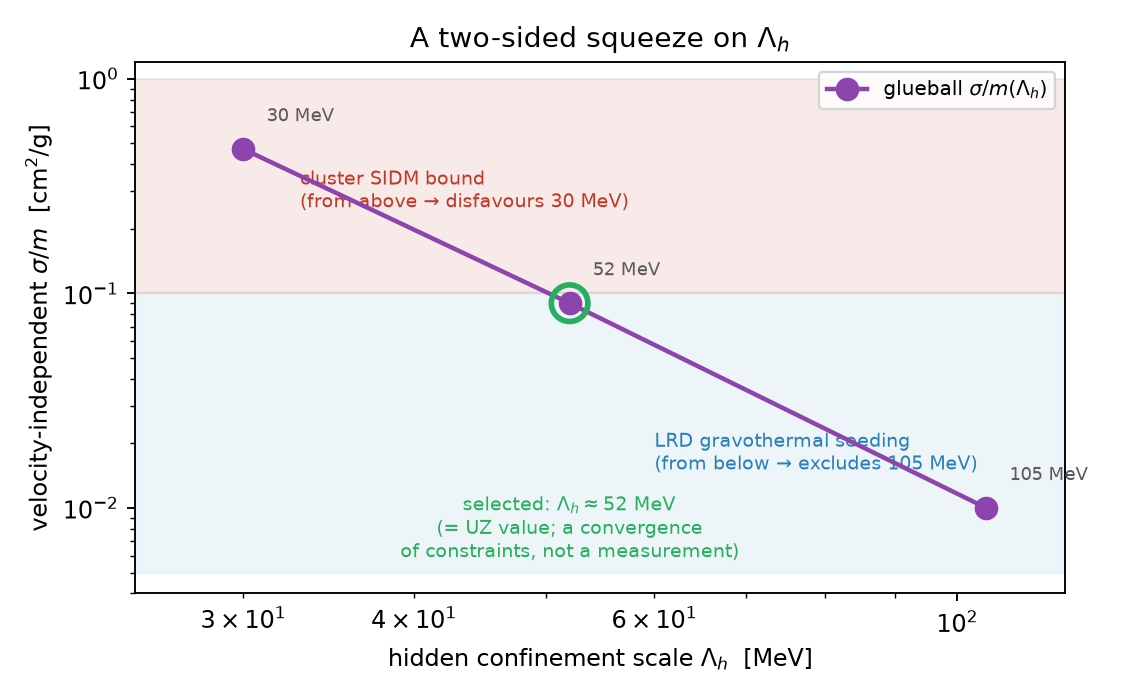
\includegraphics[keepaspectratio]{figures/fig2_pincer.png}}
\caption{The two-sided squeeze on \(\Lambda_h\). The
velocity-independent glueball self-interaction \(\sigma/m\) falls
monotonically with \(\Lambda_h\) (0.47 / 0.09 / 0.01 cm²/g at 30 / 52 /
105 MeV). Cluster SIDM bounds press from above (disfavouring 30 MeV);
Little-Red-Dot gravothermal seeding, if SIDM-driven, presses from below
(excluding 105 MeV). The window selects \(\Lambda_h \approx 52\) MeV ---
the Urban--Zhitnitsky value --- as a convergence of \emph{constraints},
not a measurement.}\label{fig:2}
\end{figure}

\begin{center}\rule{0.5\linewidth}{0.5pt}\end{center}

\section{Falsifiers}\label{sec-7}

Numbered, with current status:

\begin{enumerate}
\def\labelenumi{\arabic{enumi}.}
\tightlist
\item
  \textbf{SIDM cluster discriminator (selects UZ vs bare).} A
  cluster-scale exclusion of velocity-independent \(\sigma/m > 0.1\)
  cm²/g pushes \(\Lambda_h \gtrsim 50\) MeV, selecting the UZ-corrected
  coefficient over the bare one; conversely, a robust detection of
  velocity-\emph{dependent} self-interaction, or of velocity-independent
  \(\sigma/m\) inconsistent with the whole 0.01--0.47 cm²/g ladder, cuts
  against the glueball horn. \emph{Status: live; low-\(\Lambda_h\) end
  already at the constraint boundary.}
\item
  \textbf{Low-end \(m_X\) window (subcomponent corner).} In the
  ADM-dominant branch, a measured \(m_X \in\) 1.63--1.70 GeV is the
  glueball-subcomponent signature; \(m_X\) pinned at the top of the ECCG
  band with no shift bounds \(\xi < 0.0006\) and renders the
  subcomponent invisible. \emph{Status: awaiting an \(m_X\)
  measurement.}
\item
  \textbf{\(\Sigma m_\nu\) inheritance from Candidate C.} The glueball
  horn keeps baryogenesis on the clock channel and therefore inherits
  the D-2 neutrino squeeze in full: normal ordering with
  \(\Sigma m_\nu = 59\)--64 meV, surviving in \(\sim 1\%\) of the prior
  volume --- one DESI tightening from death. \emph{Status: live and
  near-term.}
\item
  \textbf{Lattice \(T_c/\Lambda_{\overline{\rm MS}}\) at \(N_f = 6\)
  (spec S-4).} Pins \(\Lambda_h\) within \(\sim 15\%\), deciding bare
  (28.5 MeV) vs UZ (52 MeV); disagreement with \emph{both} falsifies the
  mirror-unified transmutation identification outright. The companion
  pure-glue discharge test
  \(\rho_{\rm vac}(L) - \rho_{\rm vac}(\infty) \propto \chi_{\rm top}/(m_G L)\)
  decides the load-bearing UZ conjecture itself. \emph{Status:
  specified, external; computable with standard technology.}
\item
  \textbf{Conditional LRD falsifier (P-LRD; trigger currently unmet).}
  \emph{If} LRD follow-up establishes that the seeds require SIDM
  gravothermal collapse (i.e.~the astrophysical channels ---
  supermassive stars, super-Eddington bursts, DCBH --- are excluded),
  then within USC: \(\Lambda_h = 105\) MeV is dead as the DM scale and
  the surviving window is \(\Lambda_h \approx 30\)--52 MeV with
  baryon-boosted collapse. If LRDs are resolved astrophysically (the
  current mainstream expectation), this channel goes quiet and nothing
  in USC changes. \textbf{The trigger condition is not currently met and
  may never be}; the falsifier has not been appended to the
  pre-registration for that reason.
\end{enumerate}

A sixth, related discriminator sits one level up: with transmutation
replacing the visible-QCD amplitude hypothesis, the
dissipation-partition parameter \(b\) is unpinned and becomes
\emph{measurable} (forecast \(\sigma(\mu_0) \approx 0.05\) from DESI DR3
+ Euclid separates \(b = 0.2\) from \(b = 1\) at \(\sim 5\sigma\)),
giving a clean three-way origin discrimination: a measured
\(b \approx 0.206\) resurrects the visible-QCD hypothesis; any other
value kills it in favor of transmutation or neither.

\begin{center}\rule{0.5\linewidth}{0.5pt}\end{center}

\section{Discussion and limitations}\label{sec-8}

This section states plainly what is derived, what is matched, and what
is conjectured.

\begin{longtable}[]{@{}
  >{\raggedright\arraybackslash}p{(\linewidth - 2\tabcolsep) * \real{0.5000}}
  >{\raggedright\arraybackslash}p{(\linewidth - 2\tabcolsep) * \real{0.5000}}@{}}
\toprule\noalign{}
\begin{minipage}[b]{\linewidth}\raggedright
claim
\end{minipage} & \begin{minipage}[b]{\linewidth}\raggedright
status
\end{minipage} \\
\midrule\noalign{}
\endhead
\bottomrule\noalign{}
\endlastfoot
\(1/\alpha_h(M_{\rm Pl}) = 83.2\) confines pure hidden \(SU(3)\) at
\(\mu\) & derived \\
sensitivity \(d\ln\Lambda/d\ln\alpha = 47.5\); scale naturalized, value
log-selected & derived \\
mirror-unified \(N_f = 6\) lands in the right decade with zero new
continuous inputs & derived, and matched at the decade level \\
perturbative band 28--133 MeV, irreducibly \(O(1)\)-wide (near-conformal
loop sensitivity) & derived --- deflationary \\
\(\Lambda_h = 52\) vs 28.5 MeV discrimination & \textbf{open} ---
lattice \(T_c/\Lambda_{\overline{\rm MS}}\) (spec S-4) \\
UZ mechanism \(\rho \sim H\chi_{\rm top}/m_G\) (the law itself) &
\textbf{conjectural and contested} --- unique N1-compatible candidate;
lattice discharge test specified \\
\(\alpha_{\rm eff} = 0.25\)--0.6 for the glueball relic & derived, then
matched to the required relic abundance \\
glueball abundance & \textbf{selected}, not derived:
\(Br \approx (0.4\text{–}3)\times10^{-10}\) to \(\sim 40\%\) \\
\(\sigma/m = 0.47/0.09/0.01\) cm²/g at \(\Lambda_h = 30/52/105\) MeV &
derived \\
LRD seeding at \(\Lambda_h = 52\) MeV with \(\times 30\) baryon boost &
viability statement inside a bracket --- \textbf{not a prediction} \\
three-way convergence on \(\Lambda_h \approx 52\) MeV & convergence of
constraints, one conditional --- \textbf{not a measurement} \\
\end{longtable}

\textbf{Limitations, in order of severity.}

\begin{enumerate}
\def\labelenumi{\arabic{enumi}.}
\tightlist
\item
  \textbf{The law is conjectural.} Everything that makes this a
  \emph{dark-energy} proposal (as opposed to a natural 30--130 MeV
  hidden sector) rides on the contested UZ contact-term vacuum energy.
  We have argued it is uniquely aligned with the corpus's
  independently-forced nonlocal horizon degrees of freedom (N1) and
  evades the Casini no-go, and we have specified a cosmology-free
  lattice test --- but until that test (or an equivalent) is passed, the
  mechanism remains a conjecture and the route is incomplete.
\item
  \textbf{The output band is irreducibly \(O(1)\) perturbatively.} The
  ``zero new continuous parameters'' statement is true of the
  mirror-unification \emph{input}; the \emph{output} carries a
  factor-\(\sim 5\) loop/scheme band because \(N_f = 6\) sits near the
  conformal-window edge. The three-loop calculation was run precisely to
  tighten this and did not --- it instead exhibited a spurious IR fixed
  point marking the failure of perturbative control. We regard reporting
  this deflationary result as a feature of the program, not a defect of
  the proposal.
\item
  \textbf{The abundance dial.} The glueball horn gives up ECCG-ADM's
  explained \(\Omega_{\rm DM}/\Omega_b\) for a reheating branching ratio
  selected to \(\sim 40\%\) within a \(10^{-10}\) window. The
  mass--coupling sector is natural; the abundance is not explained.
\item
  \textbf{Sector proliferation.} The proposal adds a third hidden sector
  to the union (ECCG's \(SU(3)_H\) at \(6\times10^{12}\) GeV, the
  dark-force \(V/\varphi\) sector, and now mirror QCD at \(\sim 50\)
  MeV) --- a real cost against USC's economy claim, unless the mirror
  sector can be related to existing structure. Against this stands the
  strongest form of the economy accounting:
  \(\alpha_h(M_{\rm Pl}) = \alpha_s(M_{\rm Pl})\) (no new coupling) +
  \(N_f = 6\) (discrete) + \(Br \sim 2\times10^{-10}\) (one small
  number) + the clock jointly deliver \(\rho_{\rm DE}\)'s scale,
  \(\Omega_{\rm DM}\), \(m_{\rm DM}\), \(\eta_B\) (given
  \(\Sigma m_\nu\)), and --- via
  \(\mu^3 = (6\pi\Omega_{X0}/u_0)\,a_0 M_P^2\) --- the MOND acceleration
  scale \(a_0\) \citep{Bernal:2011wm}, connecting the Planck-scale
  coupling to galaxy rotation curves in four steps. Against ΛCDM's two
  unexplained numbers (\(\Lambda\), \(\Omega_{\rm DM}\)), that is a real
  economy, with the \(Br\) dial and the UZ conjecture as the honest
  residuals.
\item
  \textbf{Mutual exclusivity with the visible-QCD origin.} The
  transmutation origin and the corpus's existing
  \(b_{\rm QCD} = 0.2062\) visible-QCD hypothesis are mutually exclusive
  and distinguishable (§\ref{sec-7}, item 6); only one can be right, and
  current growth data (\(\mu_0 = 0.04 \pm 0.22\)) do not yet decide.
\item
  \textbf{The LRD bracket is exponentially sensitive.} The seeding
  result of §\ref{sec-6-2} spans six orders of magnitude across its
  systematic bracket and enters the pincer only conditionally. We have
  deliberately phrased it as a viability statement and kept the
  corresponding falsifier un-triggered.
\end{enumerate}

\begin{center}\rule{0.5\linewidth}{0.5pt}\end{center}

\section{Conclusion}\label{sec-9}

Dimensional transmutation converts SEDE's deepest fine-tuning --- the
origin of \(\mu = 28.5\) MeV --- into, at worst, a log-natural coupling
specification and, in the mirror-unified version, a construction with no
new continuous input at all. The honest score is: a zero-parameter
decade-level success for the scale (band 28--133 MeV, irreducibly
\(O(1)\)-wide perturbatively, with a specified lattice closer); one
contested load-bearing conjecture for the law (UZ), uniquely aligned
with the program's independently-required nonlocal horizon degrees of
freedom and equipped with a cosmology-free lattice discharge test; a
glueball dark-matter branch whose mass and coupling are natural but
whose abundance is a \(10^{-10}\)-level selection; and a set of
near-term, mutually independent probes --- cluster SIDM, a conditional
LRD bracket, the lattice ratio, DESI \(\Sigma m_\nu\), and the
growth-measured \(b\) --- that either converge on
\(\Lambda_h \approx 52\) MeV or take the identification apart. The
proposal is presented at exactly that strength and no more.

\begin{center}\rule{0.5\linewidth}{0.5pt}\end{center}

\section{Reproducibility}\label{sec-10}

All numerical claims in this paper are reproduced by the following
scripts in this repository
(\url{https://github.com/spsingularity/mu-transmutation-glueball},
\texttt{src/}):

\begin{itemize}
\tightlist
\item
  \texttt{mu\_transmutation\_check.py} --- §\ref{sec-2} coupling check
  and sensitivity; §\ref{sec-3-1} one-loop \(N_f\) scan; §\ref{sec-4} UZ
  coefficient target.
\item
  \texttt{mu\_transmutation\_steps.py} --- §\ref{sec-3-2} two-loop +
  threshold band; the \(b\)-freed sum rule and measurability forecast;
  §\ref{sec-5-4} subcomponent \(\xi\) boundaries and the \(m_X\)-shift
  window.
\item
  \texttt{mirror\_qcd\_3loop.py} --- §\ref{sec-3-3} three- and four-loop
  running, the spurious IR fixed point, and the 28--133 MeV band.
\item
  \texttt{glueball\_simp\_relic.py} --- §\ref{sec-5} decoupled-cannibal
  freeze-out, \(\alpha_{\rm eff}\) and \(\xi\)/\(Br\) bands,
  \(\Delta N_{\rm eff}\), and the §\ref{sec-6-1} \(\sigma/m\) ladder.
\item
  \texttt{glueball\_lrd\_seeding.py} --- §\ref{sec-6-2} gravothermal
  seeding calculation (halo mass function, concentration tail, collapse
  times, seed abundances).
\end{itemize}

Source assessments (dimensional transmutation, glueball-DM, and LRD
seeding) are documented in the private research hub.

\section*{Acknowledgements}\label{acknowledgements}
\addcontentsline{toc}{section}{Acknowledgements}

AI assistance: analysis and drafting were carried out with the
assistance of Claude (Anthropic); all claims were verified against the
reproducing scripts listed above.
\bibliographystyle{JHEP}
\bibliography{refs}
\end{document}
